%\documentclass[a4paper,twoside,10pt]{article}
\interfootnotelinepenalty=10000
\usepackage[USenglish]{babel} %francais, polish, spanish, ...
\usepackage[T1]{fontenc}
%\usepackage[ansinew]{inputenc}
\usepackage{color}
\usepackage{mathtools}
%\usepackage{hyperref}
\usepackage{subfig}
\usepackage{multirow, booktabs}
\usepackage{hyperref}


\usepackage{lmodern} %Type1-font for non-english texts and characters
\usepackage{algorithm}
\usepackage[noend]{algpseudocode}
\usepackage{mnsymbol}

%% Packages for Graphics & Figures %%%%%%%%%%%%%%%%%%%%%%%%%%
\usepackage{graphicx} %%For loading graphic files
\usepackage{amsmath}
\usepackage{amsthm} 
\usepackage{thmtools}
\usepackage{amsfonts}
\usepackage[all,cmtip]{xy}
\usepackage{tikz}

\usepackage{TechFront}
%\declaretheorem{Lemma}
%\declaretheorem{prop}

\newcommand{\lre}{\color{red}{\{}}

%\DeclareMathOperator{\sign}{sgn}
%\DeclareMathOperator{\coef}{coef}
%\DeclareMathOperator{\var}{var}
%\DeclareMathOperator{\eqs}{eqs}
%\DeclareMathOperator{\feas}{feas}
%\DeclareMathOperator{\UB}{UB}
%\DeclareMathOperator{\lb}{lb}
%\DeclareMathOperator{\FMcomb}{FM-comb}
%\DeclareMathOperator{\Gcomb}{Gauss-comb}
%\DeclareMathOperator{\proj}{proj}
%\DeclareMathOperator{\Pos}{Pos}
%\DeclareMathOperator{\Neg}{Neg}
%\DeclareMathOperator{\rhs}{rhs}
\newcommand{\sign}{\mathit{sgn}}
\newcommand{\coef}{\mathit{co}}
\newcommand{\var}{\mathit{var}}
\newcommand{\VAR}{\mathit{VAR}}
\newcommand{\eqs}{\mathit{eqs}}
\newcommand{\feas}{\mathit{feas}}
\newcommand{\UB}{\mathit{UB}}
\newcommand{\UBc}{\mathit{UBineq}}
\newcommand{\lb}{\mathit{lb}}
\newcommand{\lbc}{\mathit{lbineq}}
\newcommand{\FMcomb}{\mathit{FM}}
\newcommand{\Gcomb}{\mathit{GA}}
\newcommand{\proj}{\mathit{proj}}
\newcommand{\Pos}{\mathit{Pos}}
\newcommand{\Neg}{\mathit{Neg}}
\newcommand{\rhs}{\mathit{rhs}}
\newcommand{\bounds}{\mathit{bounds}}
\newcommand{\ie}{\mathcal{IE}}
\newcommand{\xx}{\mathcal{X}}
\newcommand{\vea}{\mathbf{co}}
\newcommand{\ttt}{\texttt{t}}
\newcommand{\trt}[1]{\texttt{#1}}
\newcommand{\mi}{\mathit}

\newcommand{\false}{\texttt{false}}
\newcommand{\true}{\texttt{true}}
\newcommand{\nul}{\texttt{null}}
\newcommand{\ve}{\mathbf}
%\newcommand\lhs[1]{\text{lhs}(#1)}
%\newcommand\rhs[1]{\text{rhs}(#1)}
%\newcommand\coef[1]{\text{coef}(#1)}
%\newcommand\LB[1]{\text{LB}_{#1}}
%\newcommand\UB[1]{\text{UB}_{#1}}
\newcommand{\lig}[4]{\ve{#1}\cdot\ve{#2}#3#4}
\newcommand\red[1]{\textcolor{red}{#1}}
\newcommand\blue[1]{\textcolor{blue}{#1}}
\newcommand{\set}[2]{\{\;{#1}\;|\;{#2}\;\}}
\newcommand{\odef}{\overset{\text{def.}}=}
\newcommand{\mc}{\mathcal}
\algdef{SE}[DOWHILE]{Do}{doWhile}{\algorithmicdo}[1]{\algorithmicwhile\ #1}%
\newcommand{\argmin}{\operatornamewithlimits{argmin}}
\newcommand{\StateInd}{\State\hspace{\algorithmicindent}}
\newcommand{\pr}{\mathit{PR}}
\newcommand{\prs}{\mathit{PRS}}
\newcommand{\ens}{\Leftrightarrow}

%\algdef{SE}[DOPAR]{DoPar}{doParWhile}{\algorithmicdo\textbf{ in parallel for\ }}[1]{\algorithmicwhile\ #1}%
\algdef{SE}[DOPAR]{DoPar}{doParUntil}{\algorithmicdo\textbf{ in parallel for\ }}[1]{\algorithmicuntil\ #1}%

\algdef{SE}[SUBALG]{Indent}{EndIndent}{}{\algorithmicend\ }%
\algtext*{Indent}
\algtext*{EndIndent}

\newtheorem{prop}{Proposition}
\newtheorem{lemma}{Lemma}
\newtheorem{cor}{Corollary}

\newcounter{para}
%\newcommand\mypara[1]{\par\refstepcounter{para}\textbf{\thep‌​ara\space#1\space}}
\newcommand\mypara[1]{\newline\par\refstepcounter{para}\textbf{\thepara}\space \textbf{#1} \space}
%\newcommand\mypara{\par\refstepcounter{para}\thepara\space}
%\usepackage[thmmarks,...]{ntheorem}
\newcommand{\Sec}{F}
\newcommand{\Ca}{\mi{Cap}}
\newcommand{\Vol}{\mi{V}}
\newcommand{\Weight}{\mi{W}}
\newcommand{\weight}{\mi{w}}
\newcommand{\BonjeanStations}{\mi{BS}}
\newcommand{\bonjean}{bf}
\newcommand{\Bonj}{B}
\newcommand{\shear}{\mi{sf}}
\newcommand{\Prop}{P}

\theoremstyle{definition}
%\newtheorem{example}{Example}[section]
\newtheorem*{theorem}{Theorem}

\theoremstyle{definition}
\newtheorem{examplex}{Example}[section]
\newenvironment{example}
  {\pushQED{\qed}\renewcommand{\qedsymbol}{$\triangle$}\examplex}
  {\popQED\endexamplex}
	
%\newtheoremstyle{named}{}{}{\itshape}{}{\bfseries}{.}{.5em}{\thmnote{#3}}
%\theoremstyle{named}
%\newtheorem*{namedtheorem}{Theorem}

%\begin{document}
\section{Decomposing block-angular structured system}
In the following we will describe how the structure of the considered problem can be exploited to make our projection framework perform better on large systems. Detailed pseudocode and proofs can be found in \cite{MyTechRep}. 

The considered vessel models have a \emph{(primal) block angular structure} \cite{williams}. That is, the constraint system $S$ can be divided into $k$ local subsystems, $S_1, \ldots, S_k$, using smaller, disjoint sets of variables, $X_1, \ldots, X_k$, and a global system, $S_\trt{g}$, whose constraints ``connect'' the otherwise independent subsystem by using variables from several local subsystems (see Figure~\ref{fig:decomp}). 
%
If there were no global constraints, each subsystem could be projected separately and the resulting systems could then be combined to give the projection of the original system. 
Unfortunately, the global constraints cause the local subsystems to get ``mixed'' when variables are eliminated and hence result in an increasing number of global and dense constraints, which again makes FME perform worse.

However, we can still exploit the structure of the problem. We will define and use auxiliary variables to ensure that we can project the subsystems separately without producing global constraints, before we combine the projected  subsystems and eliminate the auxiliary variables.
 
\paragraph{Using auxiliary variables to separate blocks}  
To separate and remove local variables from the global constraints, we do as follows for all subsystems $S_i$:
\begin{itemize}\itemsep0em
\item For each global constraint $c$ using variables in $S_i$, we define an auxiliary variable $z^0_{c,i}$ that equals the variables in $S_i$'s contribution to $c$. We add the equality defining $z^0_{c,i}$ to $S_i$, and we substitute with $z^0_{c,i}$ in $c$. For example, if $c: a_1x_1 + a_2x_2 + a_3x_3 + \ldots + a_kx_k \leq b$ is an inequality in $S_\trt{g}$ and $X_i = \{x_1,x_2\}$, then we add $-z^0_{c,i} + a_1x_1 + a_2x_2 = 0$ to $S_i$ and rephrase $c$ as $z^0_{c,i} + a_3x_3 + \ldots + a_kx_k \leq b$. 

We name the thusly produced subsystem $S_i^0$. 
\item Then we project $S_i^0$ w.r.t. all variables from $Y$ that are present in $S_i^0$. We do keep the auxiliary $z^0$-variables. 
Because of these auxiliary variables this only produces inequalities with variables not present in other subsystems $S_j$. 
\end{itemize}
After projecting each $S_i^0$ we can then combine the results with the rephrased, global constraints, $S_\trt{g}^0$, to create the system $\mathcal{S}$, i.e. 
\[
\mathcal{S} = S^0_\trt{g} \cup S'^0_1\cup \ldots \cup S'^0_k,
\]
where $S'^0_i$ is the projection of $S^0_i$ w.r.t. $Y\cap X_i$ for all $i\in\{1,\ldots, k\}$.
We can then eliminate all the auxiliary $z^0$-variables, $Z^0$, plus the variables in $Y$ not occurring in any $S_i$ from $\mathcal{S}$. %This results in a system equivalent to the projection of $S$ w.r.t. $Y$. %; proof can be found i \cite{MyTechRep}.

\begin{figure}[htbp]
	\centering
		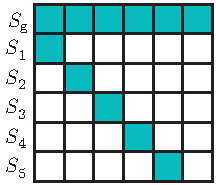
\includegraphics{figures/recursiveProjectionEs(a).pdf}
	\caption{An illustration of the coefficient matrix for a block-angular constraint system $S$ (non-zero sections coloured blue).}
	\label{fig:decomp}
\end{figure}

\paragraph{Example}
As an example, consider the block-structured problem $S$ illustrated in Figure~\ref{fig:decomp}, where $X_i=\{u_i, w_i\}$ for $i\in\{1,2,3,4,5\}$, and $S_\trt{g}=\{e,c\}$ consists of an equality defining the weighted sum, $e: - \mi{wSum} + 1u_1+ 1w_1 + 2u_2+ 2w_2 + 3u_3+ 3w_3 + 4u_4+ 4w_4 + 5u_5+ 5w_5 = 0$, and another inequality limiting the $w$s, $c: w_1 + w_2 + w_3 + w_4 + w_5\leq 20$. Assume that we want to eliminate all variables but $\mi{wSum}$, that is $Y = \bigcup_{i\in\{1,2,3,4,5\}}\{u_i,w_i\}$.

We then create the subsystems $S^0_1, \ldots, S^0_5$ and $S^0_\trt{g}$, where $S^0_i = S_i \cup 
\{-z^0_{e,i} + iu_i + iw_i = 0 \} \cup \{ -z^0_{c,i} + w_i = 0 \}$ for $i\in\{1,\ldots,5\}$, while the rephrased global inequalities are $S_\trt{g}^0 = \{-wSum + z^0_{e,1} + z^0_{e,2} + z^0_{e,3} + z^0_{e,4} + z^0_{e,5} = 0 \} \cup \{ z^0_{c,1} +z^0_{c,2} +z^0_{c,3}+z^0_{c,4}+z^0_{c,5} \leq 20\}$.   

To procure the projection of $S$ w.r.t. $Y$ we can then project $S_i^0$ w.r.t. $\{u_i, w_i\}$ for all $i\in\{1,\ldots,  5\}$, join the projections together with $S^0_\trt{g}$ in the system $\mathcal{S}$, and then project $\mathcal{S}$ w.r.t. $\set{z^0_{c,i}, z^0_{e,i}}{1\leq i\leq 5}$. {$\triangledown$}

\paragraph{Equivalent projections}
Comparing the union of the new (unprojected) subsystems, $\mathfrak{S} = S_1^0\cup\ldots\cup S_k^0\cup S_\trt{g}^0$, with the original system $S$ it is clear that
all we have done is defining auxiliary variables and substituted them in the system. Intuitively, it is therefore clear that eliminating the variables in $Y$ from $S$ is equivalent to eliminating $Y$ and the defined $z^0$-variables from $\mathfrak{S}$. 

This, in turn, is equivalent to projecting the subsystems $S^0_i$ separately w.r.t. $X_i\cap Y$, combining the resulting systems with $S^0_\trt{g}$, and then eliminate the $z^0$-variables and the remaining $Y$-variables: % The intuition behind this is, as follows: 
%
When eliminating $Y\cup Z^0$ from $\mathfrak{S}$, we can choose to first eliminate $X_1\cap Y$, then $X_2\cap Y$ up to $X_k\cap Y$, and finally $Z^0\cup Y\setminus(X_1\cup \ldots\cup X_k)$. 
Any variable in $X_1\cap Y$ has a zero-coefficient in all constraints not in $S^0_1$, and the constraints in $\mathfrak{S}\setminus S^0_1$ will therefore not be changed by the FME procedure when the variables in $X_1\cap Y$ are eliminated.  We can therefore set aside these inequalities until we have eliminated all variables in $X_1\cap Y$. Likewise, when eliminating variables in $X_i\cap Y$, no constraint from either $S_{i+1}^0\cup \ldots \cup S_k^0\cup S_\trt{g}^0$ or the already projected systems contain any variables from $X_i\cap Y$ and can hence be put aside and only included later when the variables in $Z^0\cup Y\setminus(X_1\cup \ldots\cup X_k)$ are eliminated.

Thus, the following holds. 
\begin{prop}
The projection of $S$ w.r.t. $Y$ defines the same feasible area as 
the projection of $\mathcal{S}$ w.r.t. $Z^0 \cup Y\setminus (X_1\cup \ldots \cup X_k)$.
\end{prop}

\paragraph{Further decomposition}
$\mathcal{S}$ has by construction a block-angular structure, and instead of eliminating $Z^0\cup Y\setminus(X_1\cup\ldots\cup X_k)$ immediately, if necessary, we can use further auxiliary variables to postpone ``mixing'' blocks when eliminating the remaining variables. 
To do so, we collect all subsystems into $k_1$ small groups; we have mostly used groups of size 2, 3 or 1\footnote{``Combining'' a single sybsystem corresponds to substituting a variable with a new variable, but can be done for convenience of notation.}.
For each group $i$ we do as follows:
\begin{itemize}\itemsep0em
\item We join the systems in the group into a new system, $S^1_i$. For each (rephrased) global inequality $c$ using variables occurring in $S^1_i$, we then define a variable, $z^1_{c,i}$, that equals $S^1_i$'s contribution to $c$. We then add the defining equality to $S^1_i$ and rephrase $c$ using $z^1_{c,i}$.

\item Then we project the resultant system, $S^1_i$, w.r.t. the previous, auxiliary $z^0$-variables, while we do keep the newly created $z^1$-variables.
\end{itemize} 
Subsequently we can then join the projected $S^1$-systems with the (rephrased) transverse inequalities, $S_\trt{g}^1$, and finally project the last auxiliary variables. Alternatively, we can repeat the step above step until the final projection can be done. 

\paragraph{Tree structure}
Each time we further decompose a system, we use a partitioning of the subsystems $S^l_1, \ldots, S^l_{k_l}$ to create a new level of $k_{l+1}$ subsystems, $S^{l+1}_1,\ldots, S^{l+1}_{k_{l+1}}$. This effectively creates a tree structure of smaller inequality systems, where each node is associated with a subsystem and a set of variables that should be eliminated from the system. 
Using this tree, an inequality system associated with a node is projected by recursively projecting the systems associated with the children of the node. Further, as expected, projecting the root of the tree constructed from $S$ and $Y$ as explained creates a system equivalent to the projection of $S$ w.r.t. $Y$. See Figure~\ref{fig:decomp2} and the example further below.

\begin{figure}
	\centering
		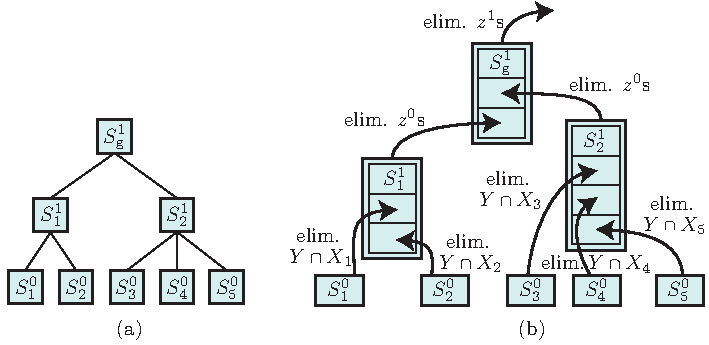
\includegraphics{figures/recursiveProjectionEs(b).pdf}
	\caption{(a) A system $S$ decomposed into a tree structure of subsystems. (b) Recursive projection of the tree-structure in (a).}
	\label{fig:decomp2}
\end{figure}

The intuition why this works is as before; projecting all $Y$ and $Z$-variables from the union of all the (unprojected) subsystems in the nodes of the tree corresponds to projecting the $Y$ variables from $S$, and because we can choose the elimination order of the variables, we only need to project the subsystems in the tree in the correct order; a rigorous proof can be found in \cite{MyTechRep}.

\begin{prop}
The projection of the system associated with the root of the tree constructed from $S$ and $Y$ w.r.t. the $Y$- and $Z$-variables as described corresponds to projecting $S$ w.r.t. $Y$.
\end{prop}

\paragraph{Example}
Consider the system from the previous example, which was decomposed into the subsystems $S^0_1, \ldots, S^0_5$ and $S^0_\trt{g}$ (Figure~\ref{fig:decomp}). Instead of projecting these subsystems as described in the previous example, we insert an additional level in the decomposition. We choose to group the five subsystems into two groups, namely $\{S^0_1, S^0_2\}$ and $\{S^0_3, S^0_4, S^0_5\}$. 
That is, we construct systems $S^1_1=\{-z^1_{e,1} + z^0_{e,1}+z^0_{e,2} = 0\}\cup \{-z^1_{c,1} + z^0_{c,1}+z^0_{c,2} = 0\}$ and $S^1_2=\{-z^1_{e,2} +z^0_{e,3}+ z^0_{e,4}+z^0_{e,5} = 0\}\cup \{-z^1_{c,2} +z^0_{c,3}+ z^0_{c,4}+z^0_{c,5} = 0\}$, and make the tree structure as in Figure~\ref{fig:decomp2}(a). The rephrased global inequalities are now $S_\trt{g}^1 = \{-wSum + z^1_{e,1} + z^1_{e,2} = 0 \} \cup \{ z^1_{c,1} + z^1_{e,2} \leq 20\}$.   
%
The projection of $S$ w.r.t. $Y$ is now made by projecting the root of the tree recursively as shown in Figure~\ref{fig:decomp2}(b). 
\\
\\
Using our previously described projection method, we obtain the projection of $S$ w.r.t. $Y$ by calling \Call{ProjectNode}{root of $T$}, where $T$ is the tree structure constructed from $S$ and $Y$, and \Call{ProjectNode}{} is as below in Algorithm~\ref{alg:decomp}. We note that due to the boundary coarsening this only approximates $\mi{proj}_Y(S)$.

\begin{algorithm}
\caption{{Using the FME framework on a decomposed, block-angular structured system.}}
\label{alg:decomp}
\begin{algorithmic}
\Function{ProjectNode}{Node $n$} 
	\State $(S,Y)\gets$ the system and variable set associated with $n$
	\If{$n$ is a leaf}
		\State \Return \Call{Project}{$S$, $Y$}\Comment Algorithm~\ref{alg:FMEF}
	\Else
		\ForAll{children $m$ of $n$}
			\State $S \gets S\cup \Call{ProjectNode}{m}$ 
		\EndFor
		\State \Return $\Call{Project}{S, Y}$ \Comment Algorithm~\ref{alg:FMEF}
	\EndIf
\EndFunction
\end{algorithmic}
\end{algorithm}

\paragraph{Other block structures} 
Using the decomposition described above, it is of course also possible to project nested block structured problems, i.e. systems that on the top-level can be divided into a global part and a number of local parts that in themselves can be further divided into local parts and a global part, and so on.  
Other block structured problems such as staircase problems can also be decomposed into a tree structure and projected using the described approach. 

\paragraph{Parallelization}
When the system $S$ is decomposed into subsystems in a tree structure as described above, the projection itself can be parallelized by maintaining a queue of not yet projected subsystems whose children have all been projected; this queue thus initially contains all leafs. 
The members of the queue are then solved independently by multiple solvers in parallel, who also add systems to the queue when the membership condition is met.
The pseudocode for this is presented below. Besides a system $S$ and a variable set $Y$, each node $n$ is associated with a number, $n_{count}$, corresponding to the number of projected children (initially set to $0$), and a system, $n_{proj}$, corresponding to the projection $\mi{proj}_Y(S)$ when it is done (initially set to $\emptyset$). 
\vspace{1mm}
\begin{algorithmic}
\Function{ParallelTreeProjection}{$S$, $Y$}
	\State Construct  tree structure $T$ from $S$ and $Y$
	\State $n_{count}\gets 0$ and $n_{proj}\gets\emptyset$ for all nodes $n$ in $T$
	\State Create a set $W$ of workers, initially idle
	\State Initialize a queue $Q$ with all leaves in $T$
	\While{$\mi{root}(T)_{proj} = \emptyset$}
		\If{$Q$ is non-empty and a worker $w\in W$ is idle}
			\State Remove first node $n$ from $Q$
			\State Use $w$ to call \Call{ProjectSingleNode}{$n$}
		\EndIf
	\EndWhile
	\State \Return $\mi{root}(T)_{proj}$
\EndFunction
\Statex
\Function{ProjectSingleNode}{Node $n$}
	\State $(S',Y')\gets$ the system and the variable set associated with $n$
	\State $S'\gets S'\cup_{m\in \mi{children}(n)} m_{proj}$ 
	\State $n_{proj}\gets$ \Call{Project}{$S'$,$Y'$} \Comment Algorithm~\ref{alg:FMEF}
	\State Increase $\mi{parent}(n)_{count}$ by one
	\If{$\mi{parent}(n)_{count} = |\mi{children}(\mi{parent}(n))|$}
		\State Add $\mi{parent}(n)$ to $Q$
	\EndIf
	\State \Return
\EndFunction
\end{algorithmic}	
\vspace{1mm}
All workers project a system using the FME framework, which again involves parallel redundancy removal, and thus it is important to only use as many resources (threads) in total as there are available.
Then, when at some point there are less nodes left to project than there are workers in $W$, the superfluous workers can pass on their resources to the remaining workers.  
%\end{document}